\documentclass[aps,reprint]{revtex4-1}
% Engine-specific settings
% Detect pdftex/xetex/luatex, and load appropriate font packages.
% This is inspired by the approach in the iftex package.
% pdftex:
\ifx\pdfmatch\undefined
\else
    \usepackage[T1]{fontenc}
    \usepackage[utf8]{inputenc}
\fi
% xetex:
\ifx\XeTeXinterchartoks\undefined
\else
    \usepackage{fontspec}
    \defaultfontfeatures{Ligatures=TeX}
\fi
% luatex:
\ifx\directlua\undefined
\else
    \usepackage{fontspec}
\fi
% End engine-specific settings
\usepackage[english]{babel}
\usepackage{csquotes}
% \usepackage[backend=biber, sortcites]{biblatex}
\usepackage{url}
\usepackage{textcomp}
\usepackage[usenames,dvipsnames,svgnames, table]{xcolor}
\usepackage[font={scriptsize}]{caption}
\usepackage{amsmath} \usepackage{amsthm} \usepackage{amsfonts}
\usepackage{amssymb}
\usepackage{enumerate}
\usepackage{tikz} \usepackage{float}
\usepackage[procnames]{listings}
\usepackage{pstool} \usepackage{pgfplots}
\usepackage{wrapfig} \usepackage{graphicx} \usepackage{epstopdf}
\usepackage{afterpage}
\usepackage{physics}
\usepackage{multirow}
\usepackage{gensymb}
\usepackage{algorithm}
\usepackage{microtype}
\usepackage[noend]{algpseudocode}
\usepackage{xcolor,colortbl}
\usepackage{microtype}
\usepackage{geometry}
\usepackage{hyperref}
\usepackage{graphicx}
\usepackage{caption}
\usepackage{subcaption}
\usepackage{lipsum}
% \usepackage{pythontex}
% \usepackage{authblk}
\usepackage{nth}
\usepackage{siunitx}
% \usepackage[toc,page]{appendix}
\floatstyle{plaintop}
\restylefloat{table}

% Custom commands
\newcommand{\unit}[1]{\:\mathrm{#1}}
\newcommand{\noref}[1]{\hyperref[#1]{\ref*{#1}}}
\newcommand{\nonref}[1]{\hyperref[]{\ref*{#1}}}
\newcommand\blankpage{%
  \null
  \thispagestyle{empty}%
  \addtocounter{page}{-1}%
  \newpage}

\newcommand{\mean}[1]{\langle #1 \rangle}

% Default fixed font does not support bold face
\DeclareFixedFont{\ttb}{T1}{txtt}{bx}{n}{7} % for bold
\DeclareFixedFont{\ttm}{T1}{txtt}{m}{n}{7}  % for normal

\newcommand\numberthis{\addtocounter{equation}{1}\tag{\theequation}}
\DeclareCaptionFont{white}{\color{white}}
\DeclareCaptionFormat{listing}{\colorbox{gray}{\parbox{\columnwidth}{#1#2#3}}}
\pgfplotsset{compat=1.14} %TODO: Setting this removed several error messages, should it be here!?


% Biber for references
% \bibliographystyle{aipauth4-1}

\begin{document}
\sisetup{detect-all}
\title{A Monte Carlo Investigation of the Ising Model}
\author{Erlend Lima}
\thanks{All code related to or referred by this paper was written in
  collaboration with Frederik J. Mellbye, along with any results it produced.
  This paper itself is written solely by the author, but was also formed through discussions with Mellbye.
 As such, similar ideas, methodology and solutions appear in Mellbye's own paper.}
\affiliation{University of Oslo, Oslo, Norway \\ Source code available at: \url{https://github.com/Caronthir/FYS3150/tree/master/Project4}}
\date{\today}

\begin{abstract}
  
The Ising model is investigated through analytical and numerical methods, where
the behavior of large scale systems are analyzed and phase transitions
found. Monte Carlo simulations were run using the Metropolis algorithm and \(10^{6}\) MC
cycles. For a $L = 2$ lattice the method is shown to reproduce analytic
expectation values. The phase transition is found to occur at a critical temperature
within $T_C = 2.25 \pm 0.05$, which includes the analytical value $\approx 2.269$ by Onsanger.
The numerical value was not computed to a higher accuracy because of time
constraints, inconsistent susceptibility values and difficulties with the code.

\end{abstract}
\maketitle
\tableofcontents
\makeatletter
\let\toc@pre\relax
\let\toc@post\relax
\makeatother

\newpage

\section{Introduction}
\label{sec:introduction}

In his 1924 PhD thesis, Ernt Ising 
solved the one dimensional Ising model devised by his adviser, Wilhelm
Lenz~\cite{weicai}. Ising showed that no phase transition can occur in one
dimension, and so triumphantly declared that no phase transition can occur in
any dimension. Lars Onsager proved otherwise when he showed that there indeed
were phase transitions in two dimensions. Even though Ising was wrong, his name
is amongst the most common names in statistical mechanics, and the model baring
his name is fundamental in the understanding of magnetic lattices.

The Ising model lends itself to numerical simulations through the
Metropolis-Hastings algorithm. This method is implemented in this paper, and is
used to study the Ising model of a ferromagnetic two dimensional lattice.
Several thermodynamic quantities are investigated, and a phase transition is
found.


In order to generalize the results the equations in this paper are scaled.
When no units are presented, energies and temperatures are scaled with $J$ and
$kT/J$, respectively. Because of the dimensionality of these quantities, the spins
and thus the system magnetic moment is dimensionless.
\section{Theory}
\label{sec:theory}

\subsection{The Ising Model}
\label{sec:isingmodel}

The Ising model is a microcanonical model which describes a lattice of discrete spins taking binary values, where each
spin interacts with its neighbors. Although simple, the Ising model is capable of modeling real
world phenomena such as ferromagnetism and phase transitions.

A lattice \(\Lambda\) is a \(d\)-dimensional graph with the nodes \(k\in\Lambda\) being spins
taking a discrete binary value, \(s_{k}\in\{-1, 1\}\). As the lattice is often
finite, its boundaries needs to be taken into account. These are treated as
periodic boundaries, where the edge on the left is connected to the edge on the
right, and the top to the bottom. For a one dimensional lattice, this topologically equivalent
to a string, while a two dimensional lattice is topologically equivalent to a torus.

For a lattice of \(N\) nodes, its energy is

\begin{equation}
  \label{eq:2}
 E = -\sum_{<kl>}^{N}J_{k,l}s_{k}s_{l} - \sum_{k}^{N}\mathcal{B}_{k}s_{k}
\end{equation}

where \(<kl>\) denotes that the sum is taken over the neighboring spins.
Between any two spins \(k, l \in \Lambda\) there is an interaction \(J_{k,l}\),
and for any spin there is the possibility of an external magnetic field with
interaction \(\mathcal{B}_{k}\). Assuming that the spin interactions are equal
for all spins and the absence of an external magnetic field, the energy
simplifies to

\begin{equation}
  \label{eq:3}
  E = -J\sum_{<kl>}^{N}s_{k}s_{l}
\end{equation}

For \(J>0\), it is favorable for neighboring spins to align, causing the
creation of magnetic domains throughout the lattice~\cite{physicslectures}.
This is called ferromagnetism. For \(J<0\), it is more favorable for spins to
point in opposite direction. The physical interpretation of this is
paramagnetism. In the remainder of this paper, it is assumed that \(J>0\).
The magnetism of the system is simply is sum over the spins,
\begin{equation}
  \label{eq:1}
  \mathcal{M} = \sum_{k} s_{k}
\end{equation}

Being microcanonical, the Ising model can be described by Boltzmann statistics.
Using this fact, it can be shown~\cite{physicslectures} that the heat capacity is
\begin{equation}
  \label{eq:4}
  C_V = \frac{\mean{E^2} - \mean{E}^2}{kT^2}
\end{equation}
and that the magnetic susceptibility is
\begin{equation}
  \label{eq:5}
  \chi = \frac{\mean{\mathcal{M}^2} - \mean{\mathcal{M}}^2}{kT}
\end{equation}
In addition, the first moment of energy can be written as
\begin{equation}
  \label{eq:6}
  \mean{E} = - \pdv{\ln{Z}}{\beta}
\end{equation}

\subsection{Phase Transitions of the Two Dimensional Ising Model}
\label{sec:phase-trans-two}
The Ising model in two dimensions without an external magnetic field was first
solved by Lars Onsager. He showed that there exists a phase transition for some
critical temperature \(T_{C}\), in contrast to the one dimensional case.

At this
temperature, the spins rapidly flip, causing spikes in thermodynamic quantities such as
heat capacity. The quantities can be modeled as~\cite{project3}


\begin{align*}
  \mean{M(T)} &\sim (T - T_C)^\beta \\
  C_V(T) &\sim |T_C - T|^\gamma \\
  \chi (T) &\sim |T_C - T|^{-\alpha}
\end{align*}
where $\alpha = 0$, $\beta = 1/8$ and $\gamma = 7/4$ are critical exponents.

The critical temperature is ideally computed for an infinite lattice size. As a
numerical simulation can never be infinite, the methods used in this paper can
only give approximations. However, there is 
a connection between the finite and infinite lattice values~\cite{physicslectures}:
\begin{align}\label{eq:crit_relation}
  T_C(L) - T_C(L = \infty) = a L^{-1/\nu}
\end{align}
where $\nu$ is found using equation (2) in~\cite{physicslectures}. The exact result for
this value is $\nu = 1$. $a$ is a constant, which can be determined by comparing
the critical temperatures for two different lattice sizes:
\begin{align}\label{eq:scalingfactor}
  a = \frac{T_C(L_1) - T_C(L_2)}{L_1^{-1/\nu} - L_2{-1/\nu}}
\end{align}
When the scaling factor $a$ is found, it can be inserted in equation~\ref{eq:crit_relation}
to find the infinite lattice value.
\subsection{Analytic Solution}
\label{sec:analytic-solution-}

For a two dimensional lattice with the above assumptions, namely the absence of a magnetic field, \(J>0\),
periodic boundaries and with a lattice size of \(L=2\) for a total of \(4\)
spins, analytical expressions for thermodynamic quantities can be found.
Labeling each spin \(s_{1}\) through \(s_{4}\), a possible spin configuration is
shown in figure~\ref{fig:22lattice}. There are \(2^{4}=16\) unique microstates, one
of which is shown in the figure. However, because of the periodic boundaries,
many of the spin states are isomorphic to each other, resulting in only five
distinct macrostates. For example, the two spin configurations in the figure are
ismorphic, as one can simply interchange the rows (or, if you will, pull the
entire lattice down through the periodic boundary) and then relabel the spins. A
complete summary is shown in table~\ref{tab:2x2values}.

\begin{figure}[H]
  \centering
  \begin{tikzpicture}[thick]
    \draw[->] (0,0) -- (0,.3)  node [label=left:{$s_1$}] {};
    \draw[->] (1,0) -- (1,.3)  node [label=right:{$s_2$}] {};
    \draw[<-] (0,1) -- (0,1.3) node [label=left:{$s_3$}] {};
    \draw[<-] (1,1) -- (1,1.3) node [label=right:{$s_4$}] {};
    \draw[-] (-.75,-.4) rectangle (1.75,1.9);

    \draw[<-] (3,0) -- (3,.3)  node [label=left:{$s_1$}] {};
    \draw[<-] (4,0) -- (4,.3)  node [label=right:{$s_2$}] {};
    \draw[->] (3,1) -- (3,1.3) node [label=left:{$s_3$}] {};
    \draw[->] (4,1) -- (4,1.3) node [label=right:{$s_4$}] {};
    \draw[-] (2.25,-.4) rectangle (4.75,1.9);
  \end{tikzpicture}
  \caption{$2 \times 2$ enumerated lattice showing two different microstates
    corresponding to the same macrostate.}
  \label{fig:22lattice}
\end{figure}


\begin{table}[H]
  \caption{Possible states and associated energies, magnetizations and degeneracies.
  The same table is also found in \cite{mortenjensen}}
  \label{tab:2x2values}
    \begin{tabular}{cccc}
      Spins up & Energy [$J$] & Magnetization & Multiplicity \\\hline
      4        & -8           & 4             & 1            \\
      3        & 0            & 2             & 4            \\
      2        & 0            & 0             & 4            \\
      2        & 8            & 0             & 2            \\
      1        & 0            & -2            & 4            \\
      0        & -8           & 4             & 1
    \end{tabular}
\end{table}

Armed with the complete knowledge of the macro states, it is feasible to compute
the partition function,

\begin{align*} \label{eq:partitionfunc}
  Z &= \sum_k e^{\beta E_k}\\
    &= 2 e^{8\beta J} + 2 e^{- 8\beta J} + 12\\
  &= 4 \cosh{(8\beta J)} + 12
\end{align*}
where \(\beta = 1/kT\) and~\eqref{eq:3} was used.


The steps proving the following relations are extensive, and not included here
for space considerations.

The mean energy is given by
\begin{align*}
  \mean{E} = -\frac{8 J \sinh{(8\beta J)}}{\cosh{(8\beta J)} + 3}
\end{align*}
and the mean of the square of the energy is given by
\begin{align*}
  \mean{E^2} = \frac{256 J^2 \cosh{(8\beta J)}}{4\cosh{8\beta J} + 12}.
\end{align*}
The energy expressions can be used to compute the heat capacity $C_V$, which
is given by
\begin{align*}
  C_V = \frac{1}{kT} \left( \mean{E^2} - \mean{E}^2 \right)
\end{align*}

Similarly, the magnetization properties are given by
\begin{align*}
  \mean{M} &= 0 \\
  \mean{M^2} &= \frac{8e^{8 J \beta} + 8}{\cosh{8\beta J} + 3}
\end{align*}
which can be used to find the susceptibility using equation~\eqref{eq:5}.

\subsection{Numerical Solution}
\label{sec:numerical-solution}

Simple systems such as the \(2\times 2\) case considered in the
previous sections lend themselves to analytical solutions, but as the systems
grow larger, it becomes increasingly difficult to find an expression for the
partition function. Instead, such systems can be solved numerically by
sidestepping the partition function completely.

This is done using Monte Carlo simulations, often through the
Metropolis-Hastings algorithm. See~\cite{physicslectures} for a detailed
explanation. A rough outline of the method is given as

\begin{enumerate}
  \item Select randomly $L^2$ spins from the \(L\times L\) lattice.
  \item Calculate the change in energy $\Delta E$ of the entire system if a randomly selected spin was to
  be flipped.
  \item Draw a random number from the uniform distribution, and compare
  \begin{align*}
    U(0,1) \leq e^{-\beta \Delta E}.
  \end{align*}
  If this is true, the spin is flipped. If this evaluates as false, do not flip
  the spin. If $\Delta E < 0$ the spin is flipped regardless, to model that physical
  systems usually tend to lower energy configurations.
\end{enumerate}

As long as the temperature is sufficiently low, the system will decrease in
energy until an equilibrium state as been reached.

Since the lattice is discrete, possible values for the change in energy \(\Delta
E\) is finite. As each flip only impacts the spin's neighbors, there are in fact
only five possible values for \(\Delta E\). It can be shown~\cite{physicslectures}
that these values are

\begin{equation*}
  \Delta E = \{-8J,\: -4J,\: 0,\: 4J,\: 8J\}
\end{equation*}

Precomputation of these values speeds up the algorithm by a noticeable amount.

\section{Method}
\label{sec:method}

\subsection{Overview}
\label{sec:overview}


The goal was to solve the Ising model numerically using the Metropolis-Hastings
algorithm as outlined in~\ref{sec:numerical-solution}. This was done completely
in C++ and partially in Julia, both producing data which was analyzed using
Python. The model was made highly flexible and user friendly, where the user could
type the parameters into a JSON-file which the C++ solver would read and solve
the corresponding model.
The Python script could then analyze the data without any need to specify the
resulting files nor their format - the script figured out this automatically.
For a more in-depth explanation of the workflow and the source code, see the
GitHub repository.

\subsection{Boundary Conditions}
\label{sec:boundary-conditions}

The fact that the C++ indexation starts at \(0\) was exploited to implement the
periodic boundary conditions of the lattice. Crossing a boundary is the same as
trying to access either a row or a column which is out of bounds. For an
\(L\times L\) lattice, attempting to access element \((0, L)\) should return
\((0,0)\), and trying to access \((0, -1)\) should return \((0, L-1)\). This is
achieved by rewriting the index \(i\) using modular arithmetic as \((i+L) \%
L\). This makes the index wrap around and satisfies the boundary conditions.

\subsection{Reaching for Equilibrium}
\label{sec:reaching-equilibrium-1}

Once a system has reached equilibrium, the expectation values of the
thermodynamic quantities will remain fairly stable about a mean, varying by some
amount determined by the temperature. As such, the equilibrium can be found by
simply looking at how the expectation values behave as a function of Monte Carlo cycles.
This analysis is done with both ordered and random initial states, repeated for different temperatures.

Another interesting quantity to investigate is the number of accepted flips as
a function of Monte Carlo cycles for different temperatures. Lower amounts of
accepted flips indicates that the system is not changing much, which is a strong
indication for whether the system is in equilibrium.


\subsection{Distribution of Energy States}
The Ising model is a discrete model with a finite state space. A system in
equilibrium will hover around the same energy state, with the variance depending
on the temperature. To investigate this, the number of occurrences of an energy
state are counted and plotted as histograms. This is done for both \(T=1\) and \(T=2.4\).

\subsection{Phase transitions} \label{sec:phase transitions}

A system at critical temperatures is characterized by abrupt changes in the
heat capacity and magnetic susceptibility. As a larger lattice more closely
approximates an infinite lattice,
the lattice size was gradually increased form \(L = 20\) to $L = 100$. The
analytic result~\cite{physicslectures} states that $T_C \approx 2.269$, and so
investigation is done 
for temperatures close to this value. It is expected that the as the lattice size
increases the approximation should improve, and the critical temperature should
therefore approach the analytical value by Onsager.

The heat capacity is plotted against temperature for temperatures around the
analytical value, and the temperature for which the heat capacity is at a
maximum is the critical temperature.  


\subsection{Parallelization}
The Ising model is so called ridiculously parallelizable, lending itself easily
to the power of parallel processing. This was implemented using MPI, but its
full power could not be leveraged due to compilation difficulties.

The source code was attempted compiled on the computing clusters
\texttt{Austur}, \texttt{Smaug}, \texttt{Abel}, \texttt{Stallo} and
\texttt{Vilje}, but all of these systems were either too outdated (did not
support C++14) or lacked the libraries (\texttt{cmake}, \texttt{armadillo} and
\texttt{jsoncpp}). Static compilation was attempted, but failed due to hardware
incompatibility. Hence, the simulations were only run on four measly cores. 

\subsection{Random number generator}
The famous Mersenne Twister PRNG was used for all the random number generation
in the code. The very long period of $2^{19937} - 1$ and fast number generation
compared to other RNGs were the main reasons for this choice.

\section{Results}
\label{sec:results}

Running the code and solving the Ising model using a multitude of different
parameters produced results which are presented here. Their interpretation is
discussed in the next section.

\subsection{Emergence of Magnetic Domains}
\label{sec:emerg-magn-doma}

The simulations should reproduce ferromagnetic behavior, i.e, magnetic domains
within the lattice. To show this, a large lattice \(L=1000\) was simulated for
200 Monte Carlo cycles, and the initial and final states plotted. These are
shown in figures~\ref{fig:initial} and~\ref{fig:final}. These are not discussed further,
and mainly serve as an aesthetic viewing pleasure.

\begin{figure}[H]
  \centering
  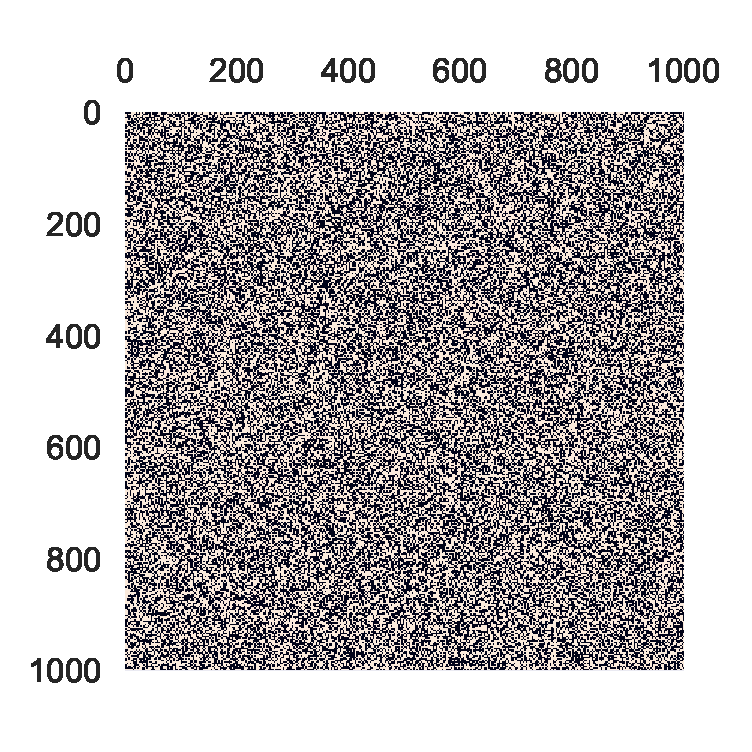
\includegraphics[width=\columnwidth]{figures/initial.eps}
  \caption{\label{fig:initial} The initial state of the lattice with randomly
    oriented spins.}
\end{figure}


\begin{figure}[H]
  \centering
  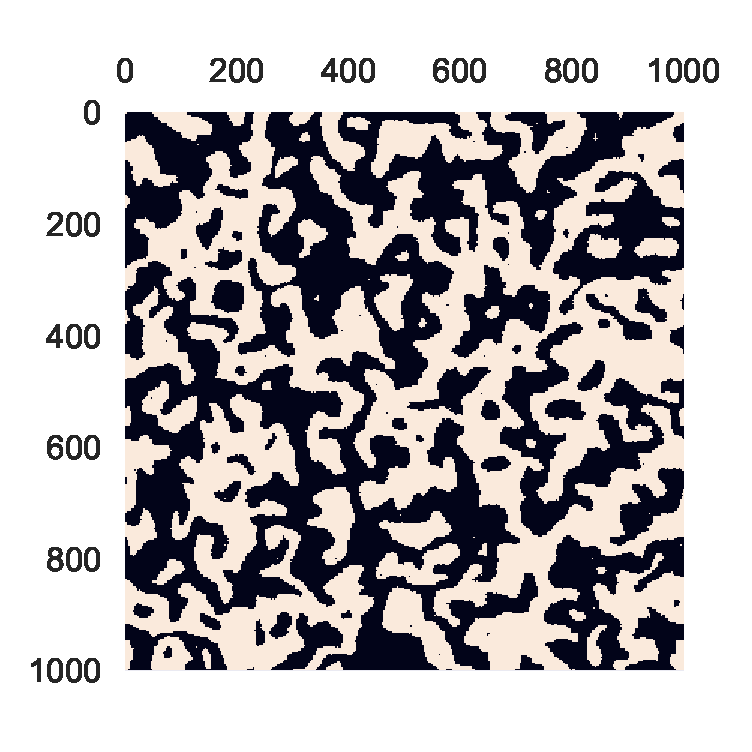
\includegraphics[width=\columnwidth]{figures/final.eps}
  \caption{\label{fig:final} The state of the lattice after 200 Monte Carlo
    cycles. Note the appearance of magnetic domains throughout the lattice.}
\end{figure}

\subsection{Numerical Solution to $2\times 2$ Lattice}
\label{sec:numer-solut-2tim}

The figures~\ref{fig:L2Ne4} through~\ref{fig:L2Ne6} illustrates how the heat
capacity changes as a function of Monte Carlo cycles for \(T = 1\).

\begin{figure}[H]
  \centering
  \includegraphics[width=\columnwidth]{figures/L2Ne4.png}
  \caption{$2 \times 2$ lattice with $M = 10^4$ MC iterations.}
  \label{fig:L2Ne4}
\end{figure}
\begin{figure}[H]
  \centering
  \includegraphics[width=\columnwidth]{figures/L2Ne5.png}
  \caption{$2 \times 2$ lattice with $M = 10^5$ MC iterations.}
  \label{fig:L2Ne5}
\end{figure}
\begin{figure}[H]
  \centering
  \includegraphics[width=\columnwidth]{figures/L2Ne6.png}
  \caption{$2 \times 2$ lattice with $M = 10^6$ MC iterations.}
  \label{fig:L2Ne6}
\end{figure}

Figures~\ref{fig:4be} to~\ref{fig:4bsusceptibility} show the expectation
values of several
thermodynamic quantities as function of temperature. The number of Monte Carlo
cycles was adapted so as to get sufficiently good results. 
\begin{figure}[H]
  \centering
  \includegraphics[width=\columnwidth]{figures/4bEnergy.eps}
  \caption{The energy as a function of temperature.}
  \label{fig:4be}
\end{figure}
\begin{figure}[H]
  \centering
  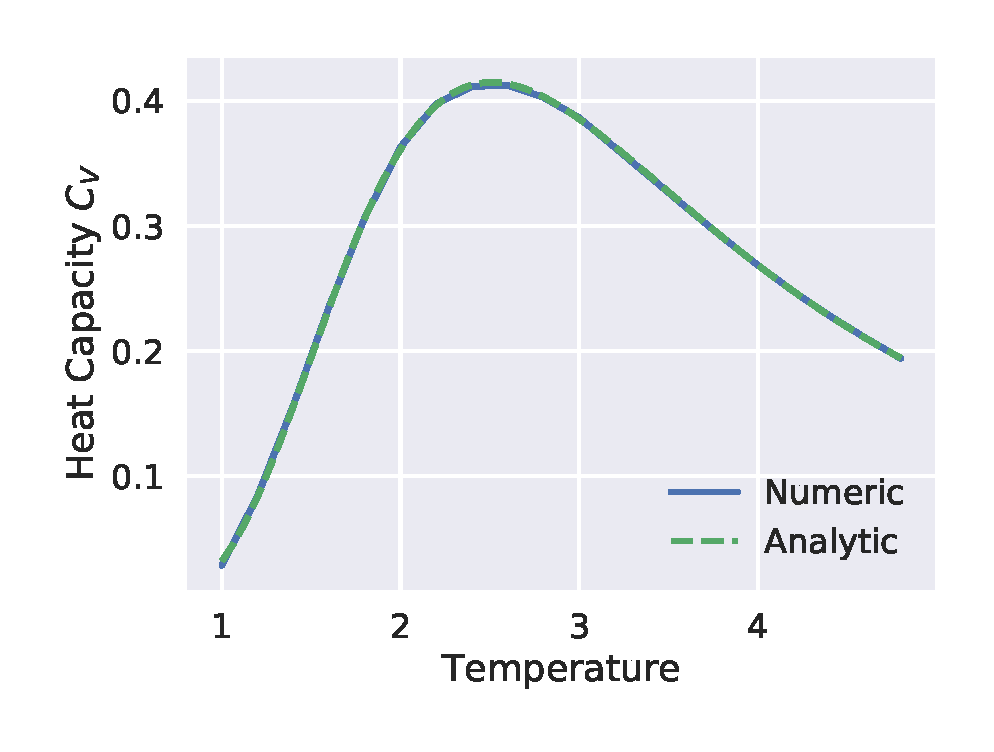
\includegraphics[width=\columnwidth]{figures/4bHeatCapacity.eps}
  \caption{The heat capacity as a function of temperature.}
  \label{fig:4bcv}
\end{figure}
\begin{figure}[H]
  \centering
  \includegraphics[width=\columnwidth]{figures/4bMagnetization.eps}
  \caption{The magnetization as a function of temperature.}
  \label{fig:4bmag}
\end{figure}
\begin{figure}[H]
  \centering
  \includegraphics[width=\columnwidth]{figures/4bSusceptibility.eps}
  \caption{The magnetic susceptibility as a function of temperature.}
  \label{fig:4bsusceptibility}
\end{figure}

\subsection{Reaching for Equilibrium}
\label{sec:reaching-equilibrium}

The figures~\ref{fig:L20T1Random} and~\ref{fig:L20T24Random} shows the energy,
magnetization and the number of spin flips as functions of temperature.
Figure~\ref{fig:4cFlips} shows how the number of flips changes as temperature increases.
\begin{figure}[H]
  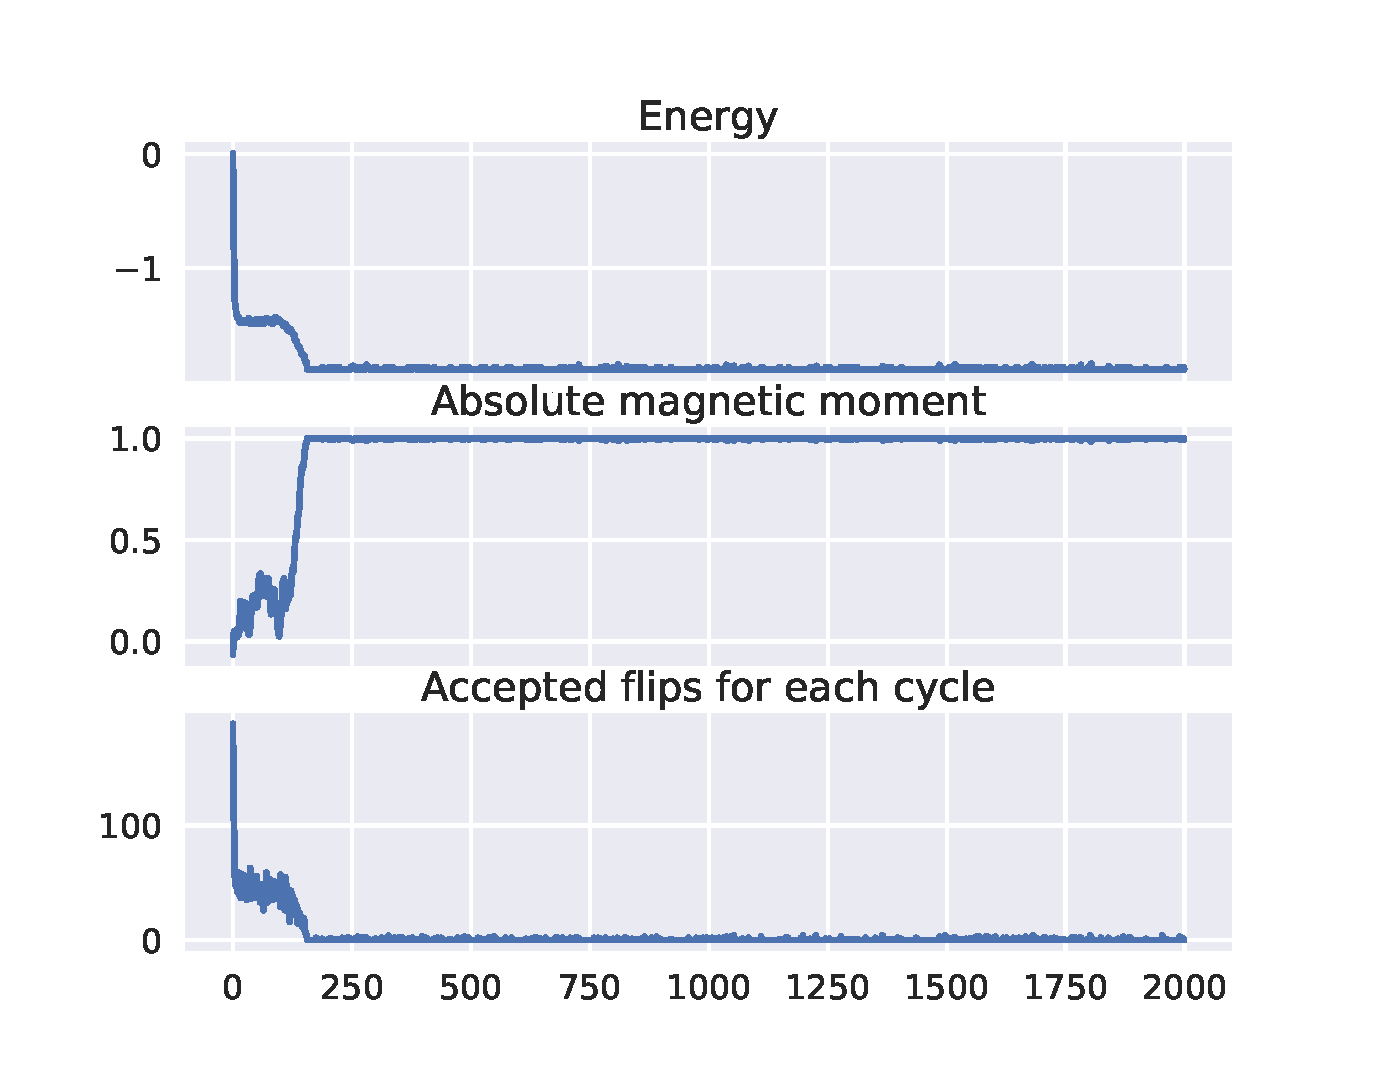
\includegraphics[width=\columnwidth]{figures/L20T1_random.eps}
  \caption{Energy, absolute magnetization and number of flips as a function of
  Monte Carlo cycles. The lattice size is $N = 20$, and the temperature $T = 1$ kT/J.}
  \label{fig:L20T1Random}
\end{figure}

\begin{figure}[H]
  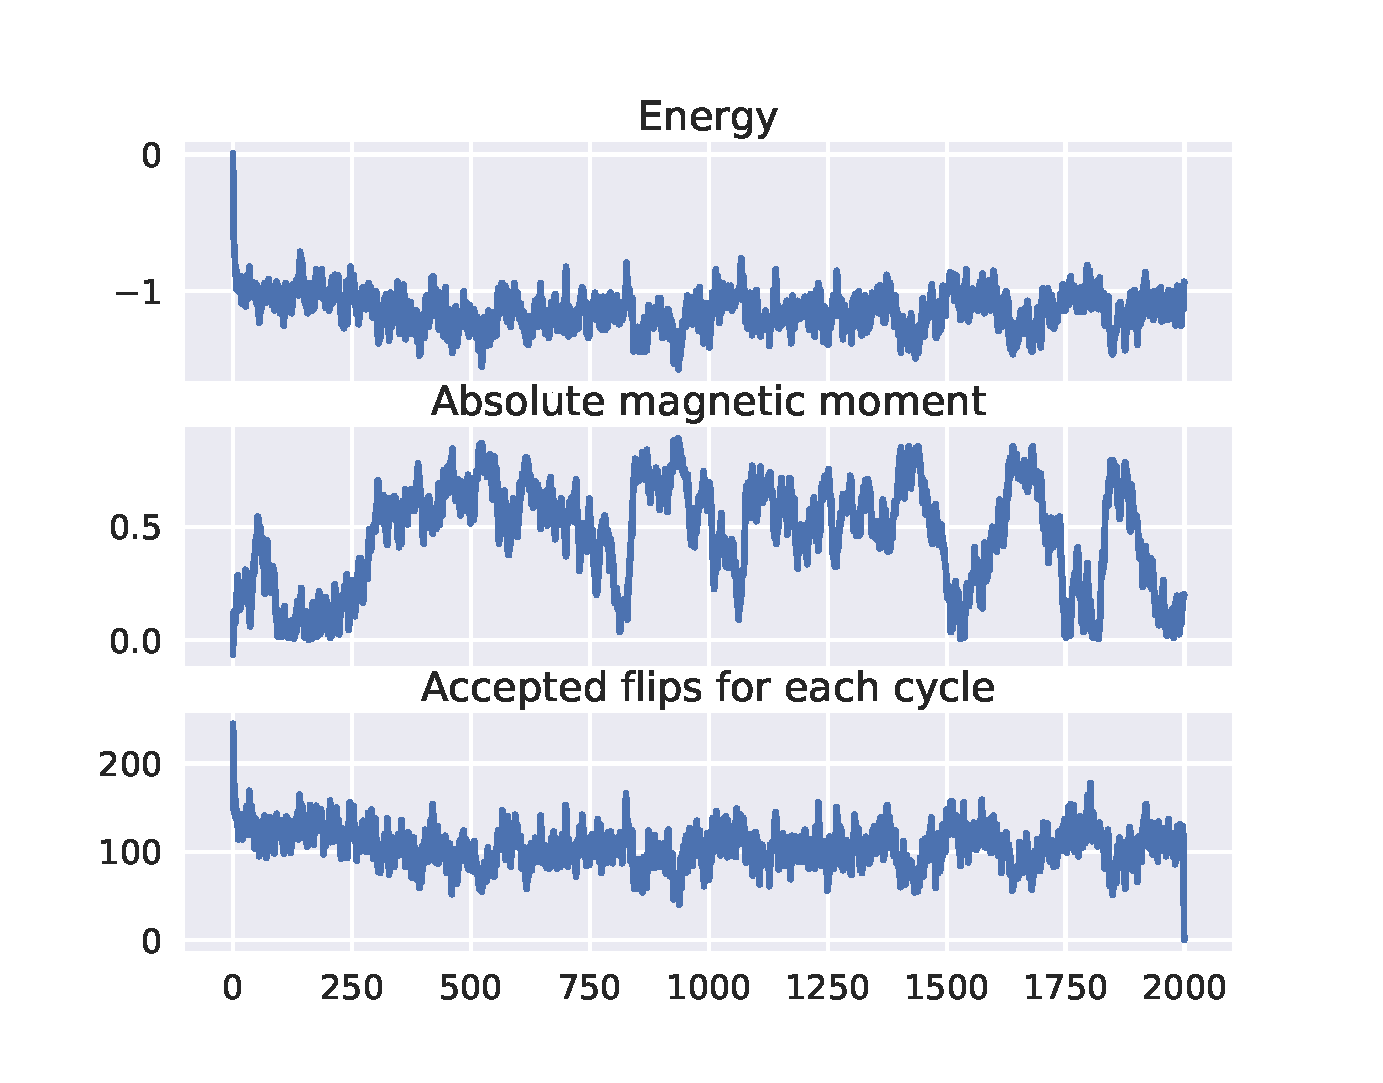
\includegraphics[width=\columnwidth]{figures/L20T2_4_random.eps}
  \caption{Initial random spins. Energy, absolute magnetization and number of flips as a function of
  Monte Carlo cycles. The lattice size is $N = 20$, and the temperature $T = 2.4$ kT/J.}
  \label{fig:L20T24Random}
\end{figure}


\begin{figure}[H]
  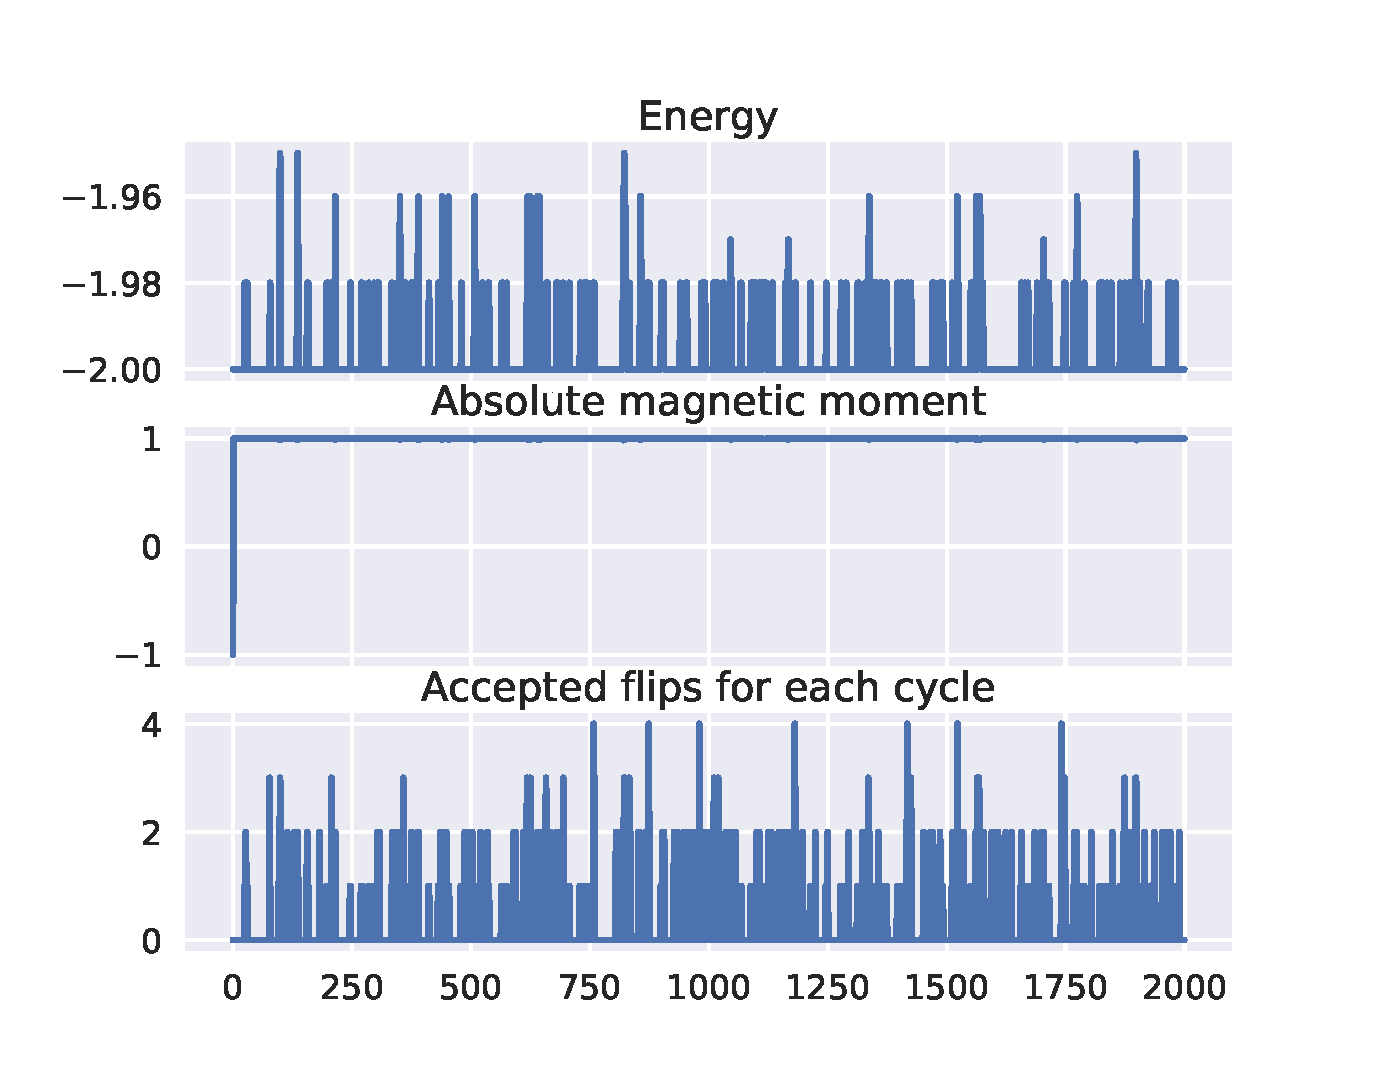
\includegraphics[width=\columnwidth]{figures/4cOrderedT1.eps}
  \caption{Initially ordered spins. Energy, absolute magnetization and number of flips as a function of
  Monte Carlo cycles. The lattice size is $N = 20$, and the temperature $T = 1.0$ kT/J.}
  \label{fig:L20T1Ordered}
\end{figure}

\begin{figure}[H]
  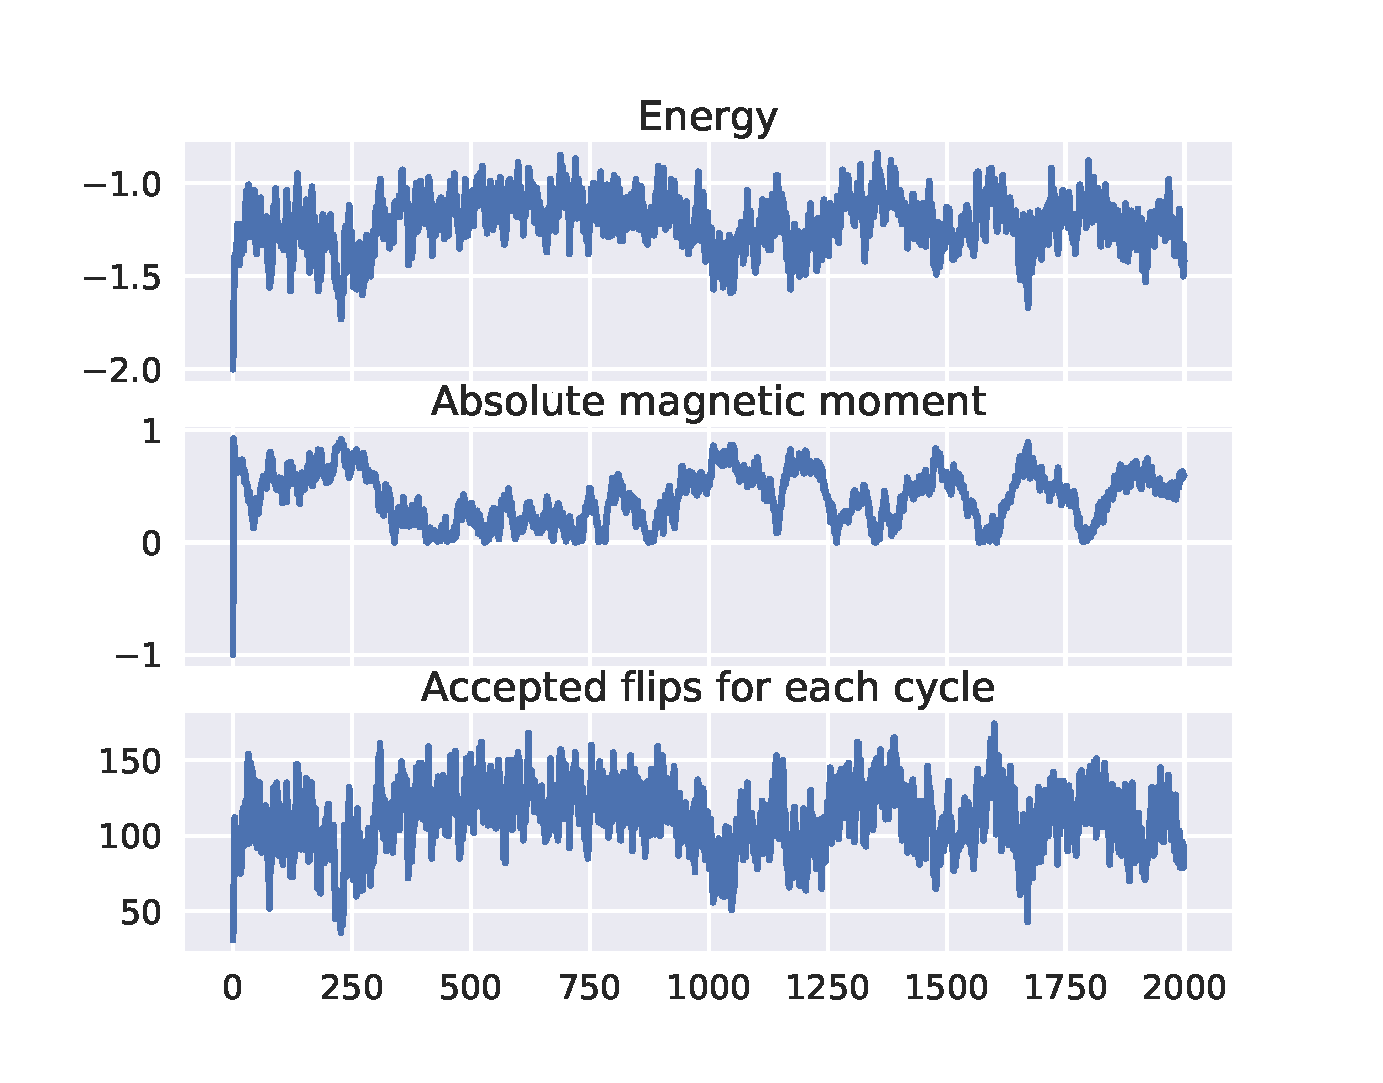
\includegraphics[width=\columnwidth]{figures/4cOrderedT24.eps}
  \caption{Initially ordered spins. Energy, absolute magnetization and number of flips as a function of
  Monte Carlo cycles. The lattice size is $N = 20$, and the temperature $T = 2.4$ kT/J.}
  \label{fig:L20T24Ordered}
\end{figure}

\begin{figure}[H]
  \includegraphics[width=\columnwidth]{figures/4c_number_of_flips.eps}
  \caption{Total number of accepted spin flips. The values are scaled with the
  maximum number to ease readability, and because only the temperature at which the
  slope changes is of interest. This was run with $10^5$ MC
  cycles for each temperature. Notice that the slope changes sign at around
  $T \approx 2.6$.}
  \label{fig:4cFlips}
\end{figure}

\subsection{Distribution of Energy States}
\label{sec:distr-energy-stat}

As there is only a finite number of discrete energy states, the number of
times a certain state occurs can be counted and represented as a histogram. This
is done for \(T=1.0\) and \(T=2.4\), shown in figures~\ref{fig:4da}
and~\ref{fig:4db}.
\begin{figure}[H]
  \centering
  \includegraphics[width=\columnwidth]{figures/4da.eps}
  \caption{\label{fig:4da} Histogram over the energy states with \(T=1.0\) kT/J.
  The variance is \(\sigma^{2} \approx 5.845\cdot 10^{-5}\)}
\end{figure}

\begin{figure}[H]
  \centering
  \includegraphics[width=\columnwidth]{figures/4db.eps}
  \caption{\label{fig:4db} Histogram over the energy states with \(T=2.4\) kT/J.
  The variance is \(\sigma^{2} \approx 0.0203\)}
\end{figure}

\subsection{The Emergence of the Phase Transition}
\label{sec:appe-phase-trans}

The phase transition is heralded by abrupt changes in the thermodynamic
quantities. For the Ising model, it is the quantities that depend on the second
derivative of the Hermholtz free energy, namely the heat capacity and magnetic
susceptibility. Figures~\ref{fig:100CVTc} to~\ref{fig:100CVTc} shows these
quantities as the lattice size changes.

\begin{figure}[H]
  \centering
  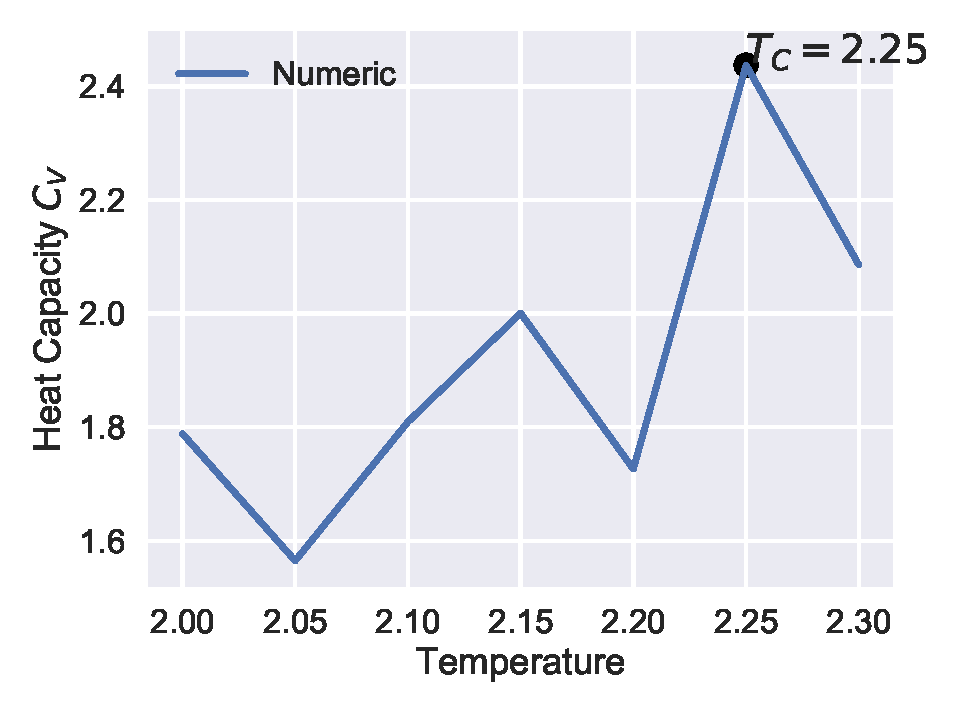
\includegraphics[width=\columnwidth]{figures/L100Cv.eps}
  \caption{\label{fig:100CVTc} Heat capacity for \(L=100\).}
\end{figure}

\begin{figure}[H]
  \centering
  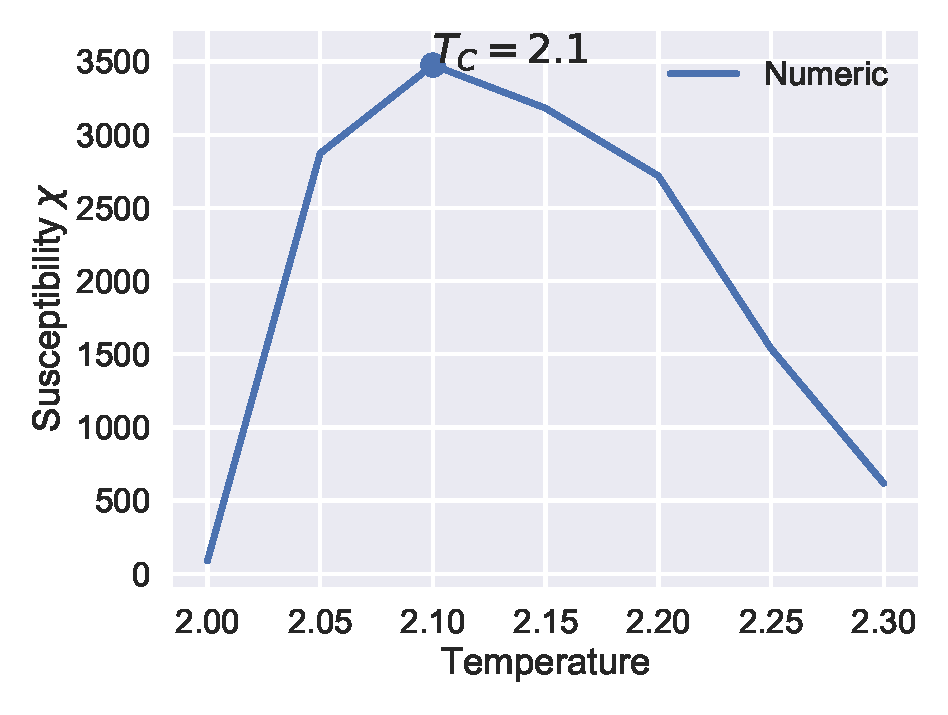
\includegraphics[width=\columnwidth]{figures/L100sus.eps}
  \caption{\label{fig:100sus} Magnetic susceptibility for \(L=100\).}
\end{figure}

\section{Discussion}
\label{sec:discussion}

\subsection{Numerical Solution to $2\times 2$ Lattice}
As a Monte Carlo simulation samples the space of possible values, running more
Monte Carlo cycles in each simulation samples more of the space, and hence gives
more accurate results. Indeed, the figures~\ref{fig:L2Ne4} to~\ref{fig:L2Ne6}
show that the numerical simulation approaches the analytical solution as the
number of Monte Carlo cycles increases. The same is true for the other
thermodynamical quantities measured, except for the energy.

The numerical solution to the energy, as shown in figure~\ref{fig:4be}, exhibit
the same shape as the analytical solution, but is linearly shifted downwards. It
is unknown why this occurs, even after scrutinizing the code.

As these results show, using about \(10^{6}\) Monte Carlo cycles is sufficient
to get results which are close enough to the analytical values. It is not
unreasonable to assume that this also holds for larger lattice sizes, and was
therefore used for the rest of the simulations. The were exceptions to this, as
if the lattice was too large, running \(10^{6}\) was infeasible.

\subsection{Reaching for Equilibrium}
\label{sec:reaching-equilibrium-2}

The studied lattice is ferromagnetic, reaching the lowest energy state when all
spins are pointing in the same direction. As a consequence, one would assume
that the systems which begin with all spins in the same state reach equilibrium
faster than when the initial spin states are random. Looking at
figures~\ref{fig:L20T1Random} to~\ref{fig:L20T24Ordered},
this is exactly what happens.

The system with initial random spins reach equilibrium after about 200 cycles.
As the temperature increases, the equilibrium is characterized by larger
fluctuations. This stems from the Boltzmann distribution, whereby a higher
temperature makes it more probable for spin flips to be accepted. This is also
reflected in the absolute magnetic moment. For low temperatures, the equilibrium
is near constant, but for higher temperatures, it varies considerably.

Comparing figures~\ref{fig:L20T1Ordered} and~\ref{fig:L20T24Ordered}, the mean
energy is more negative for the former. This stems from the fact that the
equilibrium is stable at a low energy, and any deviations from the minimal value
of \(-2\) is quickly reversed. At higher temperatures, such reversals are more
unlikely to occur, and so the systems energy is higher.


\subsection{Distribution of Energy States}
\label{sec:distr-energy-stat-2}

The two histograms in figures~\ref{fig:4da}
and~\ref{fig:4db} are entirely different beasts, at least on the surface. The
former shows an exponential distribution, while the latter a slightly skewed
normal distribution. Having the previous section about temperatures fresh in
mind, the explanation for this announces itself.

In essence, a Monte Carlo simulation samples from the state space. This space is
very large, even for small lattices, but the temperature determines how likely
each state is. At low temperatures, only the low energy states are likely to
occur - higher energy states are overwhelmingly unlikely. As previously shown,
the equilibrium state of minimum energy is quickly reached at low temperatures,
Higher energy states only occasionally appear. Since the equilibrium state is at
minimum energy, no lower energy states can occur, and the distribution becomes
exponential as in figure~\ref{fig:4da}.

Increasing the temperature makes it more likely for higher energy states to
occur, and as the equilibrium is not at the minimum energy, both lower and
higher energy states appear. However, lower energy states are favored slightly
more, making the resulting distribution normal but skewed with a heavier tail
towards lower energies. This is explains figure~\ref{fig:4db}.

\subsection{The Emergence of the Phase Transitions}
\label{sec:appe-phase-trans-2}

Lars Onsager predicted that a phase transition occurs at about \(2.269\) kT/J.
Looking at the heat capacity in figure~\ref{fig:100CVTc}, there is a peak at
\(T=2.25\). Due to the low resolution, it is only certain that the numerical
critical value occurs within the interval \([2.2, 2.3]\).

The magnetic susceptibility also should reveal a phase transition, but the plot
in figure~\ref{fig:100sus} is utter nonsense. This is surprising
considering that the numerical magnetic susceptibility coincided well with the
analytical in the \(2\times 2\) case. The reason for this is most certainly an
error in the code, but the error dodged all attempts at finding it.

If better results were found, it would be possible to use~\eqref{eq:crit_relation}. However,
due to the poor quality of the data, this was not feasible. 


\section{Conclusion}
\label{sec:conclusion}

The Ising model, although fairly simple, manages to describe many properties of
real world crystals. Analytical solutions are hard to come by, but exists for
a two dimensional \(2\times 2\) lattice. A numerical solutions using the
Metropolis-Hastings algorithm was implemented and compared to this analytical
solution, where they were in almost perfect agreement about heat capacity,
mean absolute magnetization and magnetic susceptibility, but showing a linear shift in the
mean energy.

Leaving the safe terrain of the analytic solution, the numerical solution tread
into a wilderness of large lattices, finding many weird and wonderful beasts. It
was found that the initial state of the affected how long it took for the
system to reach equilibrium. An ordered initial state reached equilibrium
faster than randomly oriented spins.

At low temperatures, the equilibrium hovered around the minimal possible
energies, while at high temperatures, the equilibrium was at higher temperatures
with far higher variation. This stems from the Boltzmann distribution, favoring
more unlikely states at higher temperatures.

Finally, it was shown that a phase transition, once deemed impossible by Ising
himself, occurred in the vicinity of \(T_{C} = 2.25\pm 0.05\). Lars Onsager
analytically showed that the critical value was at \(T_{C}\approx 2.269\),
consistent with the numerical result.

Although successful in several areas, the numerical simulations were plagued by
errors and obstacles. Due to time constraints, errors propped up in the code,
interfering with the results, hiding from wary eyes. Also, although the code was
ridiculously parallelizable, the code did not admit itself to be easily compiled
on other hardware. This would be solvable with further work.
\bibliography{references}
\end{document}

% Local Variables:
% TeX-engine: luatex
% End:
